\documentclass{article}
\usepackage{graphicx} % Required for inserting images

\title{Ants Food Selection Through Local Sampling and Distributed Decision Making}
\author{Aqsa Khan - 820165}


\begin{document}

\maketitle

\section{Introduction}
Collective systems in nature identify and exploit high-quality resources with decentralized coordination and  local communication without prior knowledge of the environment. The individual agents sense and communicate locally and the overall preference emerges from the majority's aggregated decision making. The project investigates if this can be implemented in the simulated swarm of robots. The simulation environment has two resource sites. The purpose of the experiment is to check the swam converges to the higher quality resource site using only local sampling and pheromone communication. This project is inspired by ant food-source selection mechanism. The project combines a biological literature review, a microscopic (agent-based) model, a macroscopic (population-level ODE) model, an empirically-fitted mapping between the two, and a swarm-size experiment

\section{Biological Inspiration}
This project explores the biological principles of ant colonies to address the
points in the scope of the project; a large population of simple agents that do
not have global knowledge of the environment must collectively identify and
exploit the best of several available resource sites using only local sensing and
communication. These ant colonies rely on decentralized division of labor; as
is in the project; no single ant is responsible to decide the quality of the food
source. The preference arises from the aggregate effect on many individuals.
This is precisely the property our robot swarm is designed to reproduce, using
pheromone-mediated recruitment as the core mechanism. 
\subsection{Stigmergy}
The foundational mechanism for communication and coordination among agents is stigmergy. Stigmergy is a concept inspired by termite behavior that does not communicate directly but through individuals modifying a shared environment that other individuals later sense and react to. The said modification oe the clue in the environment is called pheromone. This term was first introduced by Grasse but later Dorigo, Bonabeau, and Theraulaz later formalized this principle specifically for ant trail systems, framing pheromone deposition and evaporation as the two counteracting processes that let a colony's preference emerge and adapt over time (Dorigo et al., 2000).
\subsection{Recruitment Loop}
The underlying recruitment loop, established experimentally in the Argentine ant, consists of four stages:
\begin{enumerate}
    \item Individual ants explore initially unmarked territory largely at random.
    \item During exploration, ants that encounter a resource lay a chemical trail back toward the nest
    \item Other ants follow that trail rather than exploring independently and reinforce the trail further if they also find a resource there
    \item Trails that are not reinforced gradually evaporate and disappear(Deneubourg et al., 1990).
\end{enumerate}
This cycle of discovery, trail-laying, trail-following, and decay is directly mapped in the code in \texttt{resource\_site\_a.py} file; \texttt{discover()}, \texttt{deposit\_pheromone()}, \texttt{recruit()}, and the grid's per-timestamp evaporation.

\subsection{Collective Selection Between Competing Sources}
The classic empirical demonstration of this mechanism of producing a collective decision is the double-bridge experiment: a colony is connected to a food source by two paths of different lengths in advance. No ant has prior knowledge of the food source.The colony reliably converges on the shorter path, as the ants uses the shorter path faster in complete round trips so more pheromones are accumulated there. This recruits a positive feedback loop, that amplifies a small initially random head-start into a stable collective preference (Goss et al., 1989; Deneubourg et al., 1990). This logic was further extended to sources of quality rather than distance. It showed that the colonies modulate trail-laying intensity according to the resource encountered. The higher quality resource is reinforced more strongly and preferentially exploited (Beckers et al., 1990). Afterwards, the competitive recruitment was formalized as coupled differential equations describing population fractions committed to each trail (Nicolis \& Deneubourg, 1999). This project reproduces the quality inspired scenario; two sites varying on quality, one having qA= 0.90 and the other having qB = 0.4 and the pheromone deposit strength is set proportional to quality.  
The project uses a macroscopic ODE model to process the aggregated swarm behavior, similar to differential equation manipulation for each trail. 
\section{Problem Description}
N robots operates in a static 100x100 arena containing two resource sites. Site A has the high quality; qA = 0.9 and site B has a relatively low quality qB = 0.4. In order to keep the two trails spatially distinct; these two sites are placed in opposite corners of the arena. Robots move randomly without having any global knowledge of the site location and quality. Robots do not communicate directly, they are using pheromones to coordinate and to share their opinions. The pheromones evaporate over time proportional to the quality of site.
\subsection{Functional Requirements}
The swarm will explore the environment and detect the resource sites. Then it will estimate resource quality using probability, form opinions based on estimation and move towards consensus regarding the preferred resource. 
\subsection{Non-Functional Requirements}
The swarm shall be scalable, decentralized and fault tolerant. This means that behaviors defined by each robot is independent of N, no global coordinator and no single robot failure affects the mechanism because the sensing is purely local. 
\subsection{Assumptions}
\begin{enumerate}
    \item Each robot senses only within a small fixed radius; site detection 
    radius = pheromone sensing radius = 5.0 units in a 100 x 100 arena
    \item Robots know their own position.
    \item Communication is kept through shared pheromone grid no direct communication between two robots is considered. 
    \item Environment is static and site position and qualities are fixed.
\end{enumerate}
\section{Microscopic Model}
\subsection{Robot States}
There are three states of a robot. Each robot can only be in one state at a given instant of time; the first and initial state is undecided as the robot has not traversed the environment and know nothing about it. The second and third state is supporting A or B; the robot thinks either A is the best option or B.  Robots switch from state U to state A or from state U to state B, there is no direct transition from A to B.
\subsection{State Transition Rules}
\begin{itemize}
    \item An undecided robot within the detection radius thinks of a site adopts 
that site's opinion with probability equal to site's quality: 
$P(\texttt{adopt} \mid \texttt{discovered}) = \texttt{quality}$. This implementation is inspired by Beckers et. al's finding; adoption strength scale wits with resource values.
    \item Site quality plays a dual role, it determines the adoption probability upon discovery and the pheromone deposit strength. Consequently, a robot's internal confidence and it's trail contribution are represented by the same quantity.
    \item The undecided robot senses the average pheromone concentration within its sensing radius for both resources independently and adopts A or B with the probability proportional to that site's sensed concentration A or B. $(\texttt{RECRUITMENT\_SCALE} \times \texttt{sensed})$, with the two probabilities normalized so they never sum above 1 (competing fairly for the same undecided robot).
    \item A robot reverts to undecided with a small constant probability each timestamp (\texttt{ABANDON\_RATE}), independent of local pheromone. 
\end{itemize}
\subsection{Movement Rule}
Undecided robots perform a pure random walk and committed robots blend their random walk direction with the local gradient of their own opinion's pheromone field \texttt{GRADIENT\_BIAS}, putting them on to the stronger trails. 
\subsection{Parameter Table}
\begin{table}[htbp]
\centering
\begin{tabular}{|l|c|c|l|}
\hline
\textbf{Parameter} & \textbf{Symbol} & \textbf{Value} & \textbf{Rationale} \\ \hline
Arena size & — & $100 \times 100$ & $\sim 20\times$ sensing radius \\ \hline
Robots (development) & $N$ & $50$ & swarm-size study uses 20/50/100/200 \\ \hline
Sensing radius & $r_s$ & $5.0$ & local, non-trivial search \\ \hline
Quality A , B & $q_A, q_B$ & $0.9 , 0.4$ & clear but non-trivial gap \\ \hline
Recruitment scale & $\rho$ ($\mu$) & $0.1$ & dominant term relative to discovery \\ \hline
Abandonment rate & $\gamma$ ($\mu$) & $0.005$ & sticky opinions, stable consensus \\ \hline
Pheromone deposit & — & $\texttt{quality} \times 1.0$ & encodes quality into signal strength \\ \hline
Evaporation rate & $\delta$ & $0.02/\texttt{step}$ & approx. 35-step trail half-life \\ \hline
Gradient bias & — & $0.6$ & balance of exploration vs. exploitation \\ \hline
\end{tabular}
\caption{Swarm robotics simulation parameters.}
\label{tab:swarm_parameters}
\end{table}
\section{Macroscopic Model}
Suppose xA(t), xB(t) and xU(t) be the fraction of population supporting A,B and undecided: xU=xA-xB. The baseline model given in the project is:


The system of differential equations describing the population fractions for options $A$ and $B$ is given by:
\[
\frac{dx_A}{dt} = \alpha_A x_U + \rho_A x_A x_U - \gamma_A x_A
\]

\[
\frac{dx_B}{dt} = \alpha_B x_U + \rho_B x_B x_U - \gamma_B x_B
\]
where alpha is the discovery rate rho is a recruitment rate and gamma is opinion abandonment rate. The alpha xU represents the undecided robots stumbling on the site on their own. The recruited robots; rho xA and xB, convincing undecided ones to join up, just like in the Nicolis \& Deneubourg (1999). This macroscopic formulation implicitly assumes a well-mixed population. Gamma xA represnts robots getting tired of a site and leaving it behind. 
\section{Micro-Macro Mapping and Validation}
Macroscopic parameters; alpha, rho and gamma are fitted from agent-based simulation  trajectories via least-squares regression, exploiting the fact that ODE is linear in these parameters. Trajectories were smoothed over 20 timestep windows to reduce stochastic noise, finite differences were taken to estimate  $\frac{dx_A}{dt}$ and 
$\frac{dx_B}{dt}$, and \texttt{numpy.linalg.lstsq} was used to solve for the best-fit(alpha, rho, gamma) triple per opinion . Fitted values for one representative run(N=50, seed=40, steps=2000).
\begin{table}[h]
\centering
\begin{tabular}{|c|c|}
\hline
\textbf{Parameter} & \textbf{Value} \\
\hline
$\alpha_A$ & 0.00028 \\
\hline
$\rho_A$   & 0.00061 \\
\hline
$\gamma_A$ & 0.00057 \\
\hline
$\alpha_B$ & 0.00011 \\
\hline
$\rho_B$   & 0.00426 \\
\hline
$\gamma_B$ & 0.00202 \\
\hline
\end{tabular}
\caption{Fitted parameter values for one representative run ($N=50$, seed=42, 2000 steps).}
\label{tab:params}
\end{table}

\subsection{ODE Performance}
The ODE worked best at first when solved with scipy.integrate.solve\_ivp. The mean errors are small; 0.024 for xA and 0.030 for xB. However, the match was best early on. When the ABM simulation runs longer, the curve flattens. This causes a very small but relatively larger gap to develop. 
This gap tells exactly where the Section 5 assumptions break. The ODE assumes that any committed robot can recruit from any undecided robot, no matter where they are. But in the ABM, recruitment only happens when undecided robots wander and physically gets close to the trail. As the time passes, the pool of reachable undecided robots near trails shrinks, and the ABM's growth slows in a way the ODE can't capture as it does not know anything about space or distance. 
This is a concrete data backed answer to Section 8 question in the assignment. The micro-macro links fail when the spatial constraints and awareness start to matter. 

\begin{figure}
    \centering
    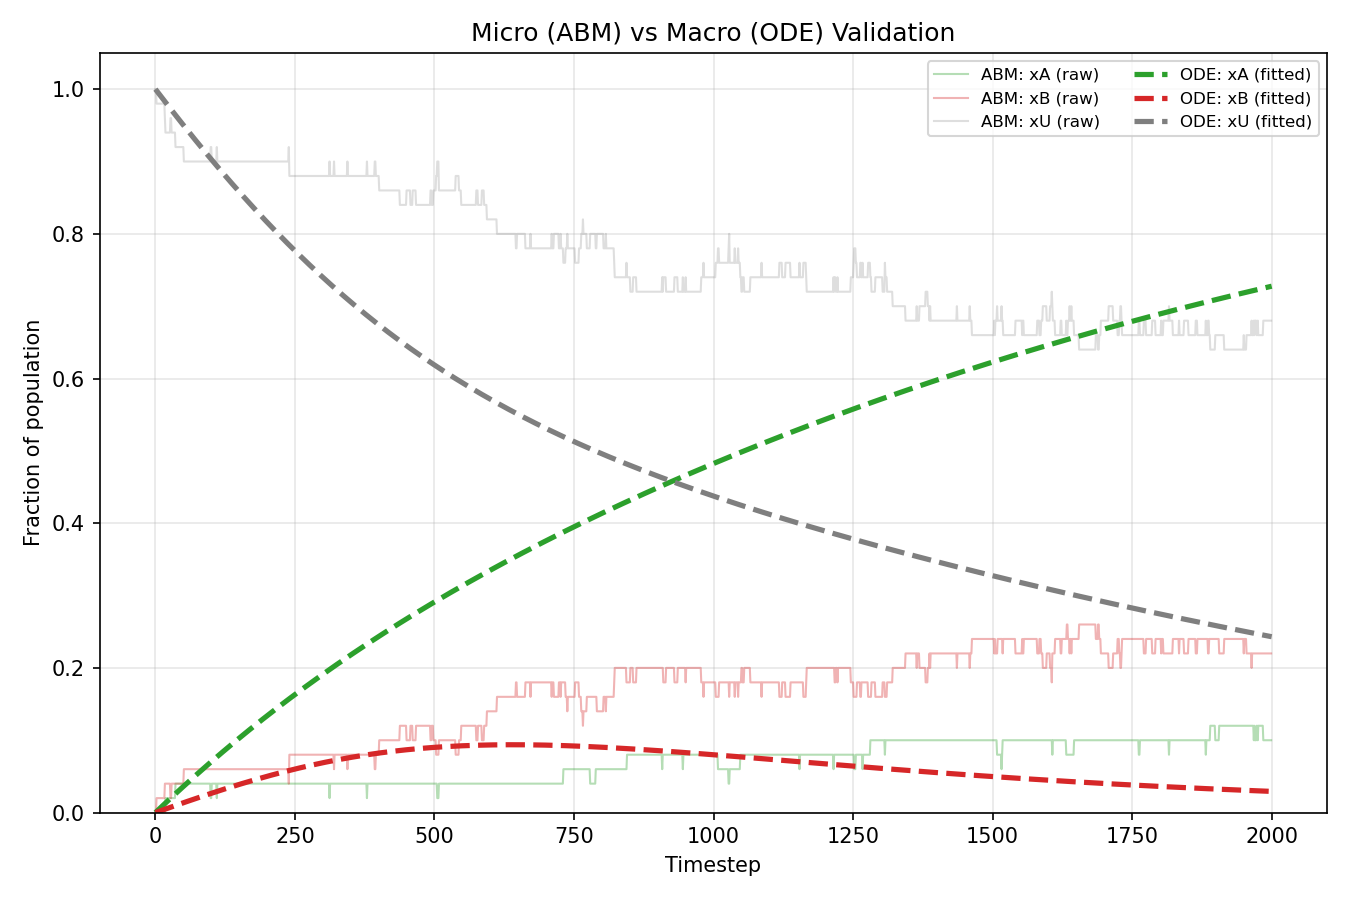
\includegraphics[width=0.5\linewidth]{macro_validation.png}
    \caption{Time evolution of ABM and fitted ODE fractions}
\end{figure}

\section{Numerical Implementation and Key Findings}
This project is implemented incrementally in python . Numpy is used for ABM, SciPy for ODE integration, pandas for experimental analysis and logging and Matplotlib for plots and figures.  
\subsection{Baseline Environment}
The baseline environment has a single site, it has no opinion and pheromones. Robots are discovering the site by randomly wandering in the environment within their sensing radius. Only $20\%$ of 50 robots discovered the site within 2000 timestamps. This can be explained by diffusive nature of random walk. This means  displacement only grows by square root of t. So with 2000 steps a robot's typical displacement is 45 units that is barely half the size of arena width. This quantifies the necessity of recruitment. This number proves; independent search is too slow and incomplete for a swarm to reliably find a food source (see Figure 2).
\begin{figure}
    \centering
    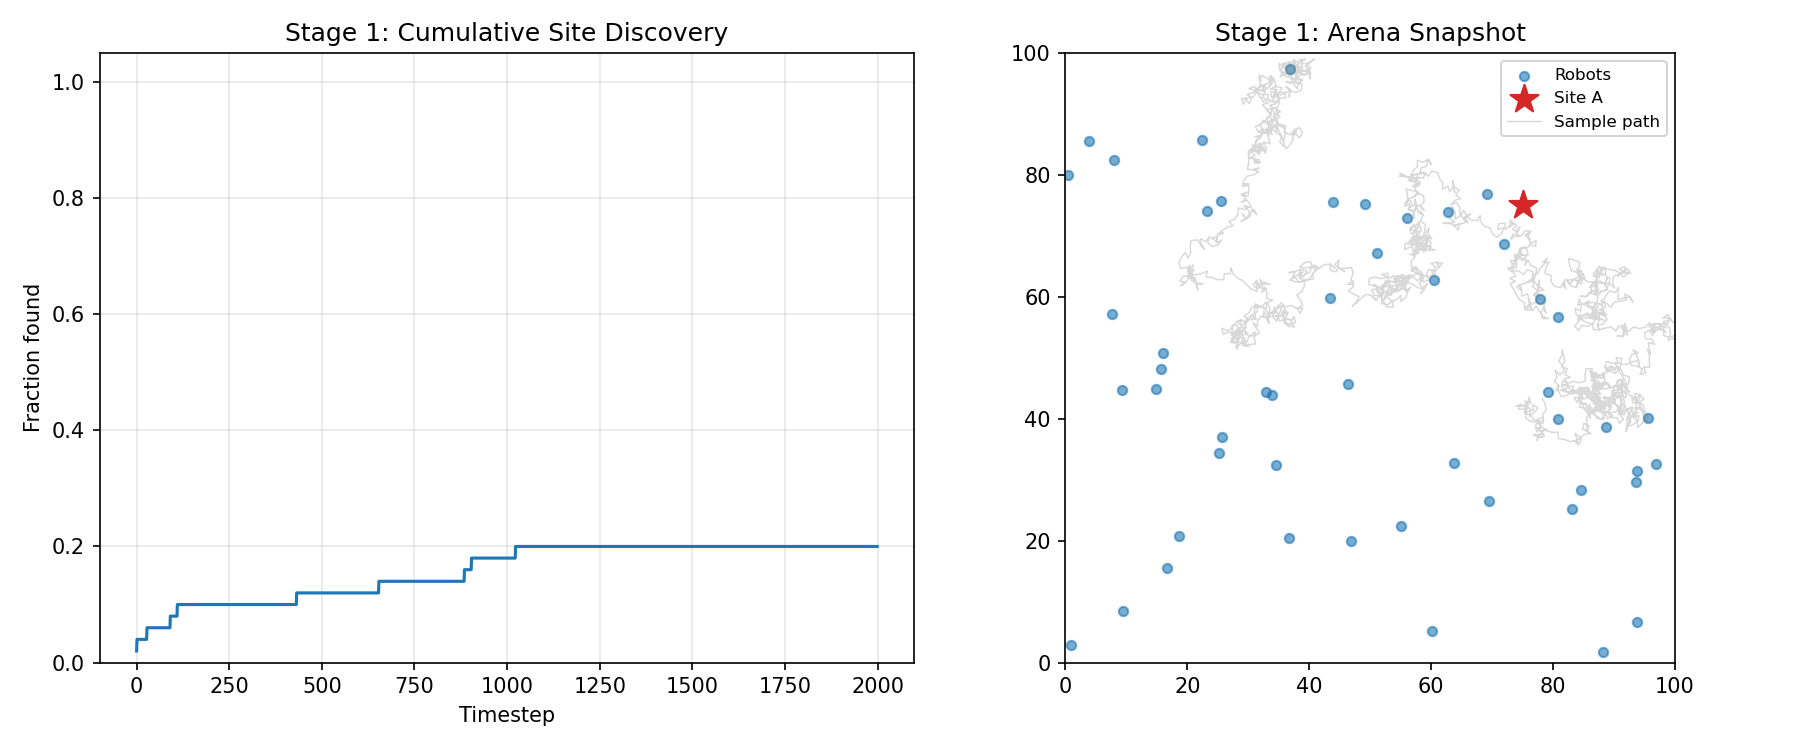
\includegraphics[width=0.5\linewidth]{basic_environment.png}
    \caption{Cumulative fraction of sites discovered in baseline environment}
    \label{fig:placeholder}
\end{figure}
\subsection{Single Site Recruitment: Exploration vs. Exploitation}
The second step in the project is to add pheromone-based recruitment for a single site. Initially plain random walk even for committed robots is used. This raised the discovery of site to $60\%$. The results however looked unrealistic. The pheromones were spread everywhere since the committed robots wandered away from the site while still depositing. Adding gradient-based movement for the committed robots fixed it and the trail matched the actual ant trail geometry. On the the hand this fix reduced the recruitment to $22\%$ because the undecided robots far from the trail were no longer recruited. This demonstrated empirical quantification for exploration-exploitation trade-off (see Figure 3). 
\begin{figure}
    \centering
    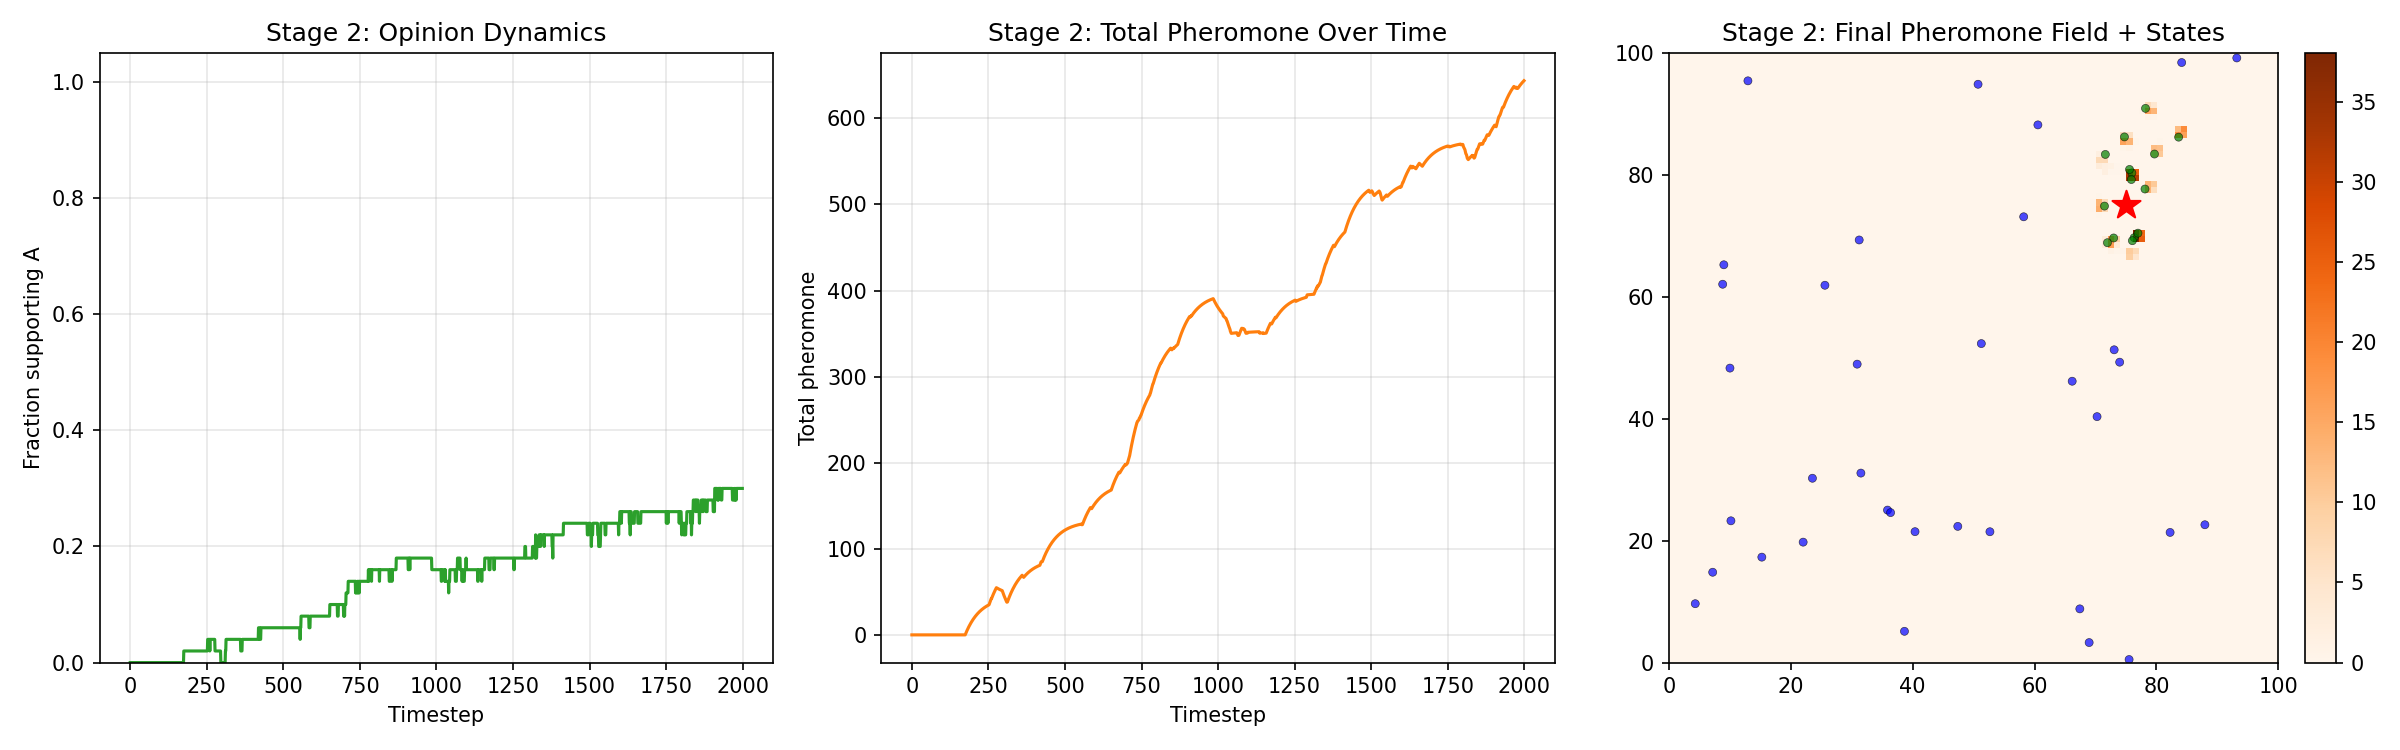
\includegraphics[width=0.5\linewidth]{single_site_pheromone.png}
    \caption{Single-site recruitment results. (a) Fraction supporting Site A over time. (b) Total pheromone accumulation over time. (c) Final pheromone field and robot states for the random-walk condition (Blue). (d) Final pheromone field and robot states for the gradient-biased condition (Red). The diffuse blue trails recruit more robots, while the localized red trails are biologically realistic but recruit fewer;quantifying the exploration-exploitation trade-off.}
    \label{fig:placeholder}
\end{figure}
\subsection{Two Competing Sites}
The third stage of the project involves two active sites A and B with qualities qA=0.9 and qB=0.4 respectively. One representative run where N=50 and steps=2000 ended with xA = $34\%$, xB= $24\%$ and xU = $42\%$. This shows the swarm exhibits a correct directional preference for higher quality site, but does not reach the full consensus within the simulated environment due to the recruitment bottleneck identified in section 7.2. The final pheromone trail demonstrates that the two trails generate separate clusters and don't not interfere geometrically (see Fig 4). 
\begin{figure}
    \centering
    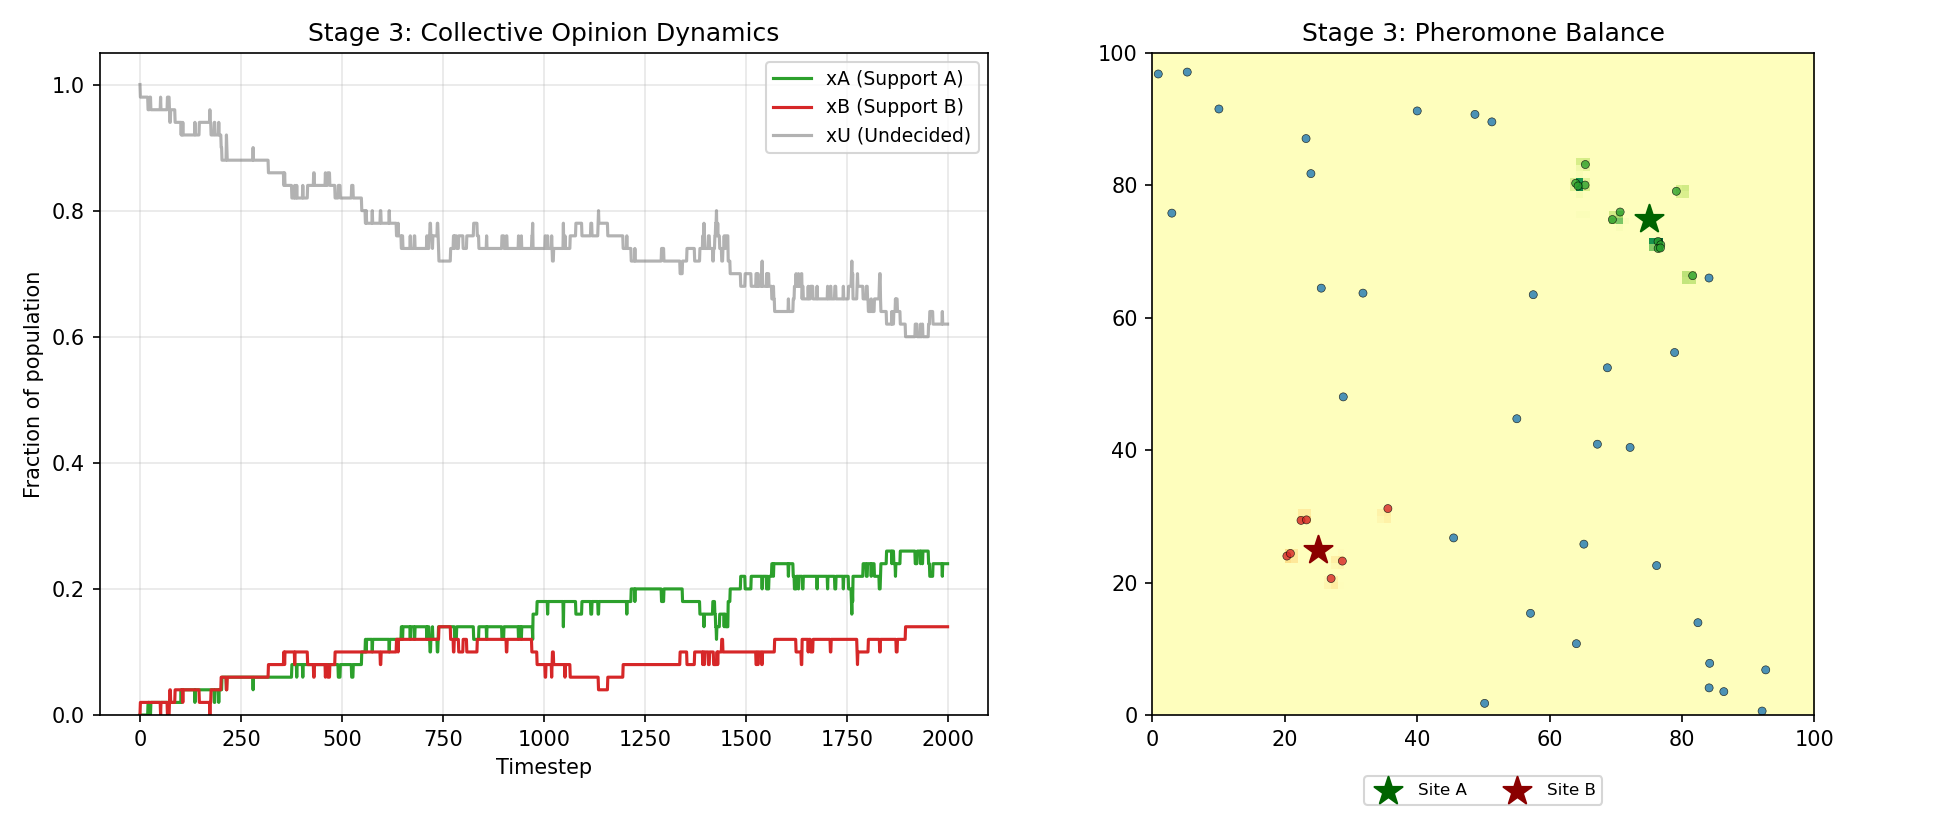
\includegraphics[width=0.5\linewidth]{two_site_competition.png}
    \caption{Two-site competition dynamics. Left panel shows the fraction of robots supporting Site A (green), Site B (red), and undecided (gray) over time. Right panel shows the population distribution as a function of pheromone balance between the two sites. The system exhibits collective decision-making as robots dynamically commit to one of the two competing sites.}
    \label{fig:placeholder}
\end{figure}
\subsection{Macro Validation}
The stage 4 of the project is already discussed in detail in Section 6 (see Fig 1)
\subsection{Swarm Sized Experiment}
The experiment is run with swarm sizes N={20,50,100,200}, using 10 random seeds for each and logging every run for 2000 timesteps. For each run, final xA, xB and xU is recorded with consensus time and decision accuracy. 

\begin{table}[htbp]
\centering
\caption{Swarm size experiment results across N = {20, 50, 100, 200}.}
\label{tab:swarm_size_results}
\begin{tabular}{|c|c|c|c|c|c|c|}
\hline
$N$ & $x_A$ & $x_B$ & $x_U$ & Decision Accuracy & Consensus Rate & Mean Time* \\
\hline
20  & 0.190 & 0.115 & 0.695 & 70\%  & 30\% & 1348 \\
\hline
50  & 0.262 & 0.140 & 0.598 & 80\%  & 30\% & 722  \\
\hline
100 & 0.369 & 0.190 & 0.441 & 90\%  & 20\% & 516  \\
\hline
200 & 0.534 & 0.321 & 0.146 & 100\% & 0\%  & n/a  \\
\hline
\multicolumn{7}{|l|}{*xA, xB, xC columns show mean values across all runs.} \\
\multicolumn{7}{|l|}{*Mean consensus time is reported only for runs where consensus occurred.} \\
\hline
\end{tabular}
\end{table}

The experiments exhibited three vivid patterns:
\begin{itemize}
    \item Bigger swarms made better decisions. Accuracy jumped from $70\%$ to $100\%$ as N increased, and the fraction of undecided robots dropped from $69.5\%$ to $14.6\%$. This happens because more robots mean more random walker covering the arena, so sites are found quickly but this evens out with more discoveries.
    \item The strick consensus metric hitting $90\%$ agreement actually dropped as N grew, hitting $0\%$ for N=100 and 200 because with enough robots, both trails become simultaneously self-sustaining, so neither ever dominates $90\%$ of the decided population, even as a swarm's overall preference becomes more reliably correct. 
    \item Consensus took less time in bigger swarms and the timesteps dropped from 1348 steps down to 516. More robots find and reinforce trails quicker, so the process speeds up in absolute terms (See Figure 5).
    \begin{figure}
        \centering
        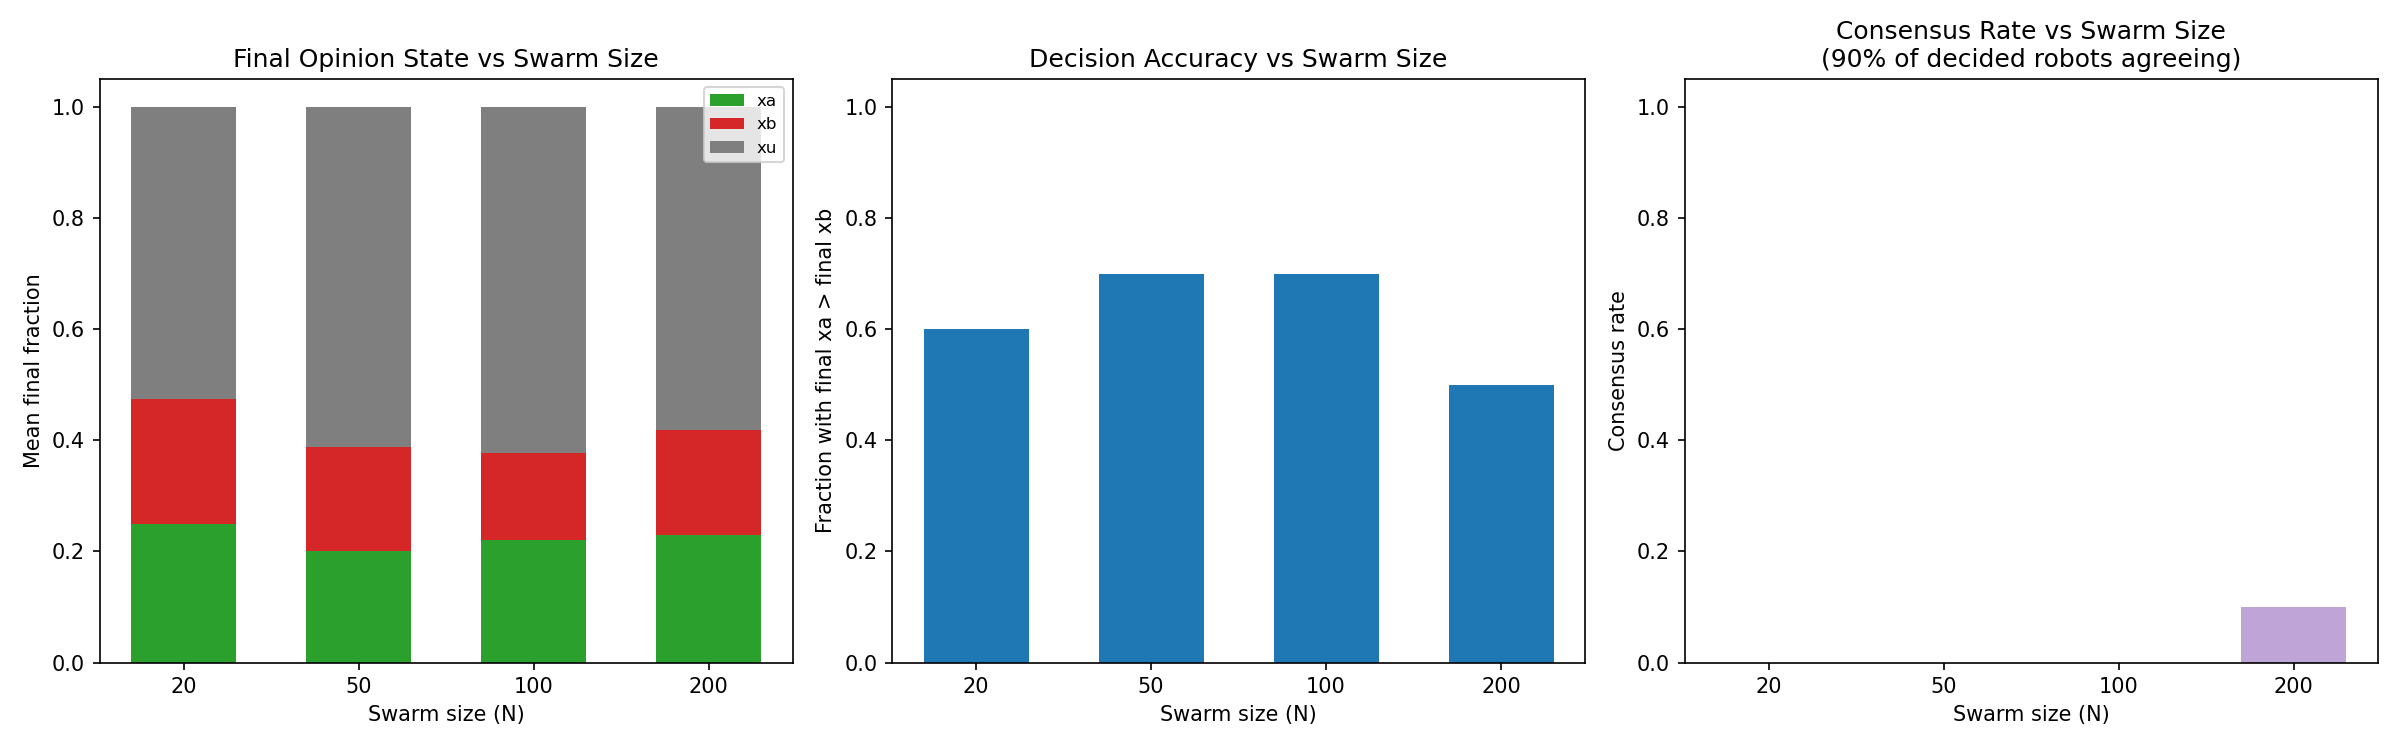
\includegraphics[width=0.5\linewidth]{stage5_swarm_size_experiments.png}
        \caption{Scaling of collective performance with swarm size}
        \label{fig:placeholder}
    \end{figure}
\end{itemize}
\section {Discussion}
\begin{itemize}
    \item Scalability: Independent of N and global counts, decision accuracy strictly improves as N grows (20 to 200) without any behavioral reconfiguration.
    \item Simplicity: Robots require zero knowledge of aggregate states, number of robots or relative site quality. There are only five local rule per timestep that each robot has to follow.
    \item Feedback Loop: The system balances fine-tuned feedback loops: positive feedback drives recruitment(via xA, xU), while negative feedback handles evaporation and abandonment. Initially, random movement breaks the tie between identical sites, and site quality naturally determines which of those random trails grow into stable paths. 
    \item Stigmergic Communication: The robots don not talk directly. They coordinate indirectly through shared pheromone field, leaving clues in the environment for others to pick up.
    \item Exploitation vs Exploration: There is a delicate balance between exploration and exploitation: while localized trails allow robots to hone onto a target effectively. Focused navigation limits their overall reach compared to a more diffused exploratory search.
    \item Micro-Macro Mapping: Both levels are connected empirically. The divergence between them driven by spatial locality yields valuable insights rather than indicating model failure. 
    \item Swarm Behavior: Individual robots having no prior knowledge of sites and tracks, yet a robust swarm-level preference for the superior site emerges. This strengthens reliability on N out of simple local interactions.
\end{itemize}
\section{Conclusion}
This project implemented a full micro-macro pipeline for collective resource selection, grounded in a specific, well-documented biological mechanism (ant pheromone recruitment) rather than an arbitrary swarm algorithm. Several results were not assumed in advance but discovered empirically through the stimulation itself: individual random search is demonstrably too slow to rely on alone. Spatially, realistic trails trade off against recruitment reach; the swarm reliably prefers the higher-quality site but does not always reach strict consensus within a bounded arena and time horizon. The microscopic mean field model agrees with the microscopic stimulation only until spatial locality causes the ABM saturate below the ODE's prediction. Decision accuracy and consensus rate are genuinely different, sometimes oppositely trending, measures of collective success as swarm size scales. These findings connects to standard building blocks of swarm robotics, with each principle supported by a specific reproducible measurement from this project's own simulations rather than by assertion alone.
\section{References}
\begin{enumerate}
    \item Beckers, R., Deneubourg, J.L., Goss, S., \& Pasteels, J.M. (1990). Collective decision making through food recruitment. Insectes Sociaux, 37(3), 258-267.
    \item Deneubourg, J.L., Aron, S., Goss, S., \& Pasteels, J.M. (1990). The self-organizing exploratory pattern of the Argentine ant. Journal of Insect Behavior, 3(2), 159-168.
    \item Dorigo, M., Bonabeau, E., \& Theraulaz, G. (2000). Ant algorithms and stigmergy. Future Generation Computer Systems, 16(9), 851-871.
    \item Goss, S., Aron, S., Deneubourg, J.L., \& Pasteels, J.M. (1989). Self-organized shortcuts in the Argentine ant. Naturwissenschaften, 76, 579-581.
    \item Grasse, P.P. (1959). La reconstruction du nid et les coordinations interindividuelles chez Bellicositermes natalensis et Cubitermes sp. La theorie de la stigmergie: essai d'interpretation du comportement des termites constructeurs. Insectes Sociaux, 6, 41-83.  
    \item Helbing, D., Keltsch, J., \& Molnar, P. (1997). Modelling the evolution of human trail systems. Nature, 388, 47-50.
    \item Lerman, K., \& Galstyan, A. (2002). Mathematical model of foraging in a group of robots: Effect of interference. Autonomous Robots, 13, 127-141.   
    \item Nicolis, S.C., \& Deneubourg, J.L. (1999). Emerging patterns and food recruitment in ants: an analytical study. Journal of Theoretical Biology, 198(4), 575-592. 
    \item Payton, D., Daily, M., Estowski, R., Howard, M., \& Lee, C. (2001). Pheromone robotics. Autonomous Robots, 11(3), 319-324.
    
\end{enumerate}
\end{document}


